\chapter{HASIL DAN PEMBAHASAN}

\section{Isi Bab Hasil dan Pembahasan}
\blindtext

\section{Melampirkan Tabel}
\blindtext \ref{table:nilai}.

\begin{table}[H]
\centering
\caption{Parameter kelulusan tugas akhir}
\begin{tabular}{ clc }
\hline
\textbf{No.} & \textbf{Parameter } & \textbf{Nilai} \\
\hline
1. & Penulisan & A \\
2. & Penulisan & A \\
\hline
\end{tabular}
\label{table:nilai}
\end{table}


%Berikut adalah contoh tabel yang dicetak secara horizontal
%gunakan package longtable
%Dapat dibuat dulu di https://www.tablesgenerator.com/ lalu dipindah
\begin{landscape}
\begin{longtable}{p{3.5cm}cllllll}
\caption{Contoh Tabel Mendatar yang Panjang dan Lebar}\\
\hline
\textbf{Provinsi} & \textbf{Kode Wilayah} & \textbf{Singkatan Umum} & \textbf{ISO} & \textbf{Pulau} & \textbf{Ibu Kota} & \textbf{Gubernur} \\ \hline
\endfirsthead

\multicolumn{4}{l}{\bfseries \tablename\ \thetable{} -- Lanjutan dari halaman sebelumnya}\\
% \begin{center}
% % {{\bfseries \tablename\ \thetable{} -- Lanjutan dari halaman sebelumnya}} \\
% \end{center}
\hline
\textbf{Provinsi} & \textbf{Kode Wilayah} & \textbf{Singkatan Umum} & \textbf{ISO} & \textbf{Pulau} & \textbf{Ibu Kota} & \textbf{Gubernur} \\ \hline

\endhead

\hline
\endfoot

\endlastfoot



Aceh & 11 & Aceh & ID-AC & Sumatera & Banda Aceh & Achmad Marzuki \\
Sumatera Utara & 12 & Sumut & ID-SU & Sumatera & Medan & Edy Rahmayadi \\
Sumatera Barat & 13 & Sumbar & ID-SB & Sumatera & Padang & Mahyeldi Ansharullah \\
Riau & 14 & Riau & ID-RI & Sumatera & Pekanbaru & Syamsuar \\
Jambi & 15 & Jambi & ID-JA & Sumatera & Jambi & Al Haris \\
Sumatera Selatan & 16 & Sumsel & ID-SS & Sumatera & Palembang & Herman Deru \\
Bengkulu & 17 & Bengkulu & ID-BE & Sumatera & Bengkulu & Rohidin Mersyah \\
Lampung & 18 & Lampung & ID-LA & Sumatera & Bandar Lampung & Arinal Djunaidi \\
Kepulauan Bangka Belitung & 19 & Babel & ID-BB & Sumatera & Pangkalpinang & Ridwan Djamaluddin \\
Kepulauan Riau & 21 & Kepri & ID-KR & Sumatera & Tanjungpinang & Ansar Ahmad \\
Daerah Khusus Ibukota Jakarta & 31 & DKI Jakarta & ID-JK & Jawa & Tidak ada & Heru Budi Hartono \\
Jawa Barat & 32 & Jabar & ID-JB & Jawa & Bandung & Ridwan Kamil \\
Jawa Tengah & 33 & Jateng & ID-JT & Jawa & Semarang & Ganjar Pranowo \\
Daerah Istimewa Yogyakarta & 34 & DIY & ID-YO & Jawa & Yogyakarta & Hamengkubuwana X \\
Jawa Timur & 35 & Jatim & ID-JI & Jawa & Surabaya & Khofifah Indar Parawansa \\
Banten & 36 & Banten & ID-BT & Jawa & Serang & Al Muktabar \\
Bali & 51 & Bali & ID-BA & Nusa Tenggara & Denpasar & I Wayan Koster \\
Nusa Tenggara Barat & 52 & NTB & ID-NB & Nusa Tenggara & Mataram & Zulkieflimansyah \\
Nusa Tenggara Timur & 53 & NTT & ID-NT & Nusa Tenggara & Kupang & Viktor Laiskodat \\

Kalimantan Barat & 61 & Kalbar & ID-KB & Kalimantan & Pontianak & Sutarmidji \\
Kalimantan Tengah & 62 & Kalteng & ID-KT & Kalimantan & Palangka Raya & Sugianto Sabran \\
Kalimantan Selatan & 63 & Kalsel & ID-KS & Kalimantan & Banjarbaru & Sahbirin Noor \\
Kalimantan Timur & 64 & Kaltim & ID-KI & Kalimantan & Samarinda & Isran Noor \\
Kalimantan Utara & 65 & Kaltara & ID-KU & Kalimantan & Tanjung Selor & Zainal Arifin Paliwang \\
Sulawesi Utara & 71 & Sulut & ID-SA & Sulawesi & Manado & Olly Dondokambey \\
Sulawesi Tengah & 72 & Sulteng & ID-ST & Sulawesi & Palu & Rusdy Mastura \\
Sulawesi Selatan & 73 & Sulsel & ID-SN & Sulawesi & Makassar & Andi Sudirman Sulaiman \\
Sulawesi Tenggara & 74 & Sultra & ID-SG & Sulawesi & Kendari & Ali Mazi \\
Gorontalo & 75 & Gorontalo & ID-GO & Sulawesi & Gorontalo & Hamka Hendra Noer \\
Sulawesi Barat & 76 & Sulbar & ID-SR & Sulawesi & Mamuju & Akmal Malik \\
Maluku & 81 & Maluku & ID-MA & Maluku & Ambon & Murad Ismail \\
Maluku Utara & 82 & Malut & ID-MU & Maluku & Sofifi & Abdul Ghani Kasuba \\
Papua & 91 & Papua & ID-PA & Papua & Jayapura & Lukas Enembe \\
Papua Barat & 92 & Pabar & ID-PB & Papua & Manokwari & Paulus Waterpauw \\
Papua Selatan & 93 & Pasel & — & Papua & Merauke & Apolo Safanpo \\
Papua Tengah & 94 & Papteng & — & Papua & Nabire & Ribka Haluk \\
Papua Pegunungan & 95 & Papeg & — & Papua & Wamena & Nikolaus Kondomo \\
Papua Barat Daya & 96 & PBD & — & Papua & Sorong1 & — \\ \hline
\label{table:tabelpanjanglebar}
\end{longtable}
\end{landscape}


		\subsection{Subsubbab 2 2}
		\blindtext

	\section{Subab 3}
	\blindtext \ref{fig:komputer}

\begin{equation}
    x+2 = 159
\end{equation}
\blindtext

%Berikut adalah contoh gambar yang dicetak secara horizontal
\begin{landscape}
   \begin{figure}[t]
        \centering
        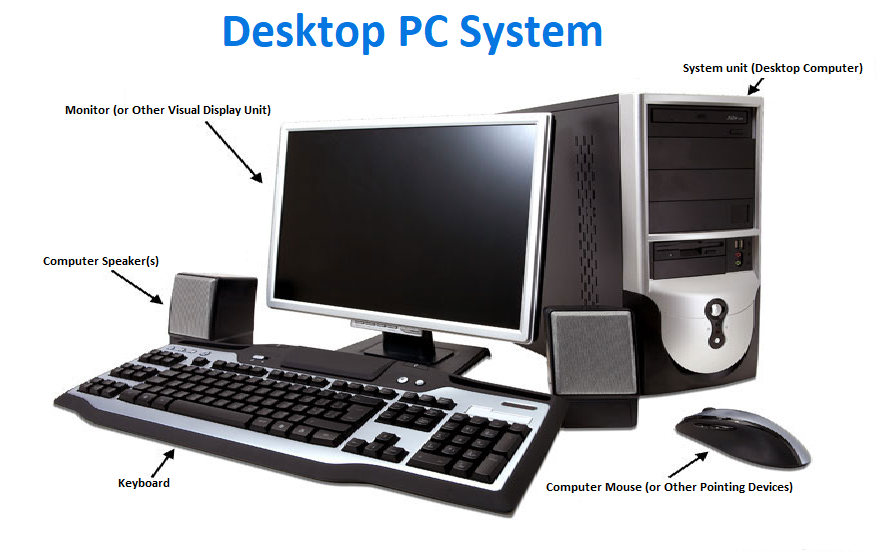
\includegraphics[width=18cm, height=12cm]{gambar/contoh-gambar-miring.png}
        \caption{Contoh Gambar Komputer}
        \label{fig:komputer}
    \end{figure}
\end{landscape}

